\part{Methods}

\chapter{Theoretical Framework}
\label{cha:theory}

\section{Outline}

\chapter{Biomedical Named Entity Recognition}

The identification of gene names is an importnat steps in patent retrieval

Research efforts in biomedical text mining and gene entity recognition have focused on scientific abstracts \cite{RodriguezEsteban2016TextMP}.

\chapter{Biomedical Data Integration}

Data Integration is a constantly growing and evolving part of science, engineering and biomedical computing, as labs often need to combine and consolidate each other`s data \cite{Bernstein2008InformationII}.

First, the data must be understood and then prepared for the data integration process employing data cleansing and standardization \cite{Bernstein2008InformationII}.

The two broad goals of the data integration process are to increase the completeness and conciseness of data \cite{Bleiholder2009DataF}.
Completeness is increased by adding more data sources \cite{Bleiholder2009DataF}.
Conciseness is achieved by removing redundant data \cite{Bleiholder2009DataF}.

Integrated information systems provide a unified view of heterogeneous data sources by querying the underlying data sources and combining the results. This paper utilizes an integration scenario with a three-step data integration process, as shown in Figure \ref{fig:data-integration-process} \cite{Bleiholder2009DataF}.

\begin{figure}
	\begin{center}
	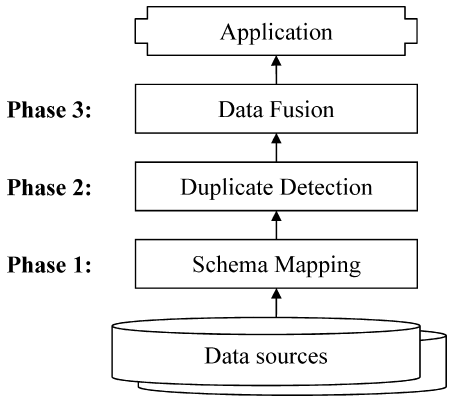
\includegraphics[width=13cm]{./figures/dataIntegrationProcess.PNG}
	\caption[A data integration process]{A data integration process \cite{Bleiholder2009DataF}}
	\label{fig:data-integration-process}
	\end{center}
\end{figure}

\section{Data Translation}

Although some databases cover the same subject, they may are heterogeneous and uses different schemas \cite{Bernstein2008InformationII}. 
To cope with this kind of heterogeneity, one needs a mediated schema that covers the desired subject matter \cite{Bernstein2008InformationII}. 
First, one needs to identify corresponding attributes that describe the information items in the sources \cite{Bleiholder2009DataF}. 
The result of this step is known as \textit{schema mapping} \cite{Bleiholder2009DataF}. 
The data gets then mapped from the source schema into the new mediated schema \cite{Bernstein2008InformationII}.
Data Translation aims to bridge the schematic heterogeneities by transforming data from multiple data sources to conform to the global schema \cite{Bleiholder2009DataF}.

Two approaches are common to bridge schematic heterogeinities: schema integration and schema mapping \cite{Bleiholder2009DataF}.

Schema integration requires to generate a new schema that is complete and correct with respect to the source schemata \cite{Bleiholder2009DataF}.

Schema mapping assumes a given target schema. A set of correspondences between elements of a source schema and elements of the target schema are generated to specify the data transformation \cite{Bleiholder2009DataF}.

The objectives of both schema integration and schema mapping are to transform the data of the sources into a global schema \cite{Bleiholder2009DataF}.



\textit{Usage of XML.} Often data sources are incomplete with respect to the target schema, with each source missing some information that the others provide. XML is a semi-structured data format where each data element is tagged. Therefore, only those element, whose values are known to need to be included. This ability to handle variations in the content is driving the increased usage of XML in the data integration context \cite{Bernstein2008InformationII}.

\textit{Data Cleansing.} When the same or similar information is contained in multiple places, some of the occurrences are likely inconsistent. An initial step of the data integration process is to inspect data sources for such kind of inconsistencies.

\section{Identity Resolution}

The second step of the data integration process is identity resolution, also known as record linkage, duplicate detection or object identification \cite{Bleiholder2009DataF}.
This process is also referred to in the literature as data merging, data consolidation or duplicate detection \cite{Bleiholder2009DataF}.
The objective is overcoming semantic heterogeneity by integrating information into one single and consistent representation \cite{Bleiholder2009DataF}.
The objective is to identify multiple representations of the same real-world object \cite{Bleiholder2009DataF}.
To identify duplicate representations of the same real-world object, one needs to compare each pair of objects using a similarity measure and threshold \cite{Bleiholder2009DataF}.
If a pair of objects has a higher similarity measure than the given threshold, it is a duplicate \cite{Bleiholder2009DataF}.

\textit{Effectiveness and Efficiency.} The process of identity resolution embarks two main difficulties: effectiveness and efficiency \cite{Bleiholder2009DataF}.
The quality of the similarity measure and the choice of the threshold are the determining factors for effectiveness \cite{Bleiholder2009DataF}.
Similarity measures are domain-independent \cite{Bleiholder2009DataF}.
A low threshold will result in a high recall since all duplicates are found, but low precision since many nonduplicate pairs are declared duplicates \cite{Bleiholder2009DataF}.
On the contrary, a high threshold will result in high precision but low recall \cite{Bleiholder2009DataF}.
Since calculating and storing all pairs of objects for large datasets can become an obstacle, Efficiency is an issue \cite{Bleiholder2009DataF}.
An intelligent partitioning overcomes this obstacle \cite{Bleiholder2009DataF}.
More than two representations which share the same object-ID are referred to in the literature as \textit{duplicate clusters} \cite{Bleiholder2009DataF}.

Naumann2010AnIT
With increasing volume of data, data quality problems abound \cite{Naumann2010AnIT}.

\textbf{String Matching.}

%Tokenizing Jaccard Similarity //
%de.uni_mannheim.informatik.dws.winter.similarity.string.TokenizingJaccardSimilarity
%Sorensen Dice //
%info.debatty.java.stringsimilarity.SorensenDice
%Levenshtein //
%de.uni_mannheim.informatik.dws.winter.similarity.string.LevenshteinSimilarity
%Cosine //
%info.debatty.java.stringsimilarity.Cosine

Given two sets of strings \textit{X} and \textit{Y}, the aim is to determine all pairs of strings \textit{(x,y)} where \textit{x} $\in$ \textit{X} and \textit{y} $\in$ \textit{Y}, such that \textit{x} and \textit{y} refer to the same entity \cite{Doan2012PrinciplesOD}. \\
\\
\textbf{Accuracy Challenge.} Accurate string matching is challenging to realize since the strings referring to the same entity are often very different. The causes for differences between strings include typing error, different formatting conventions, custom abbreviation, shortening of strings, different names or shuffling parts of the strings. Similarity measures provide a solution to the accuracy challenge by taking a pair of strings \textit{(x,y)} as input and return a score in the range between \textit{[0,1]}: The higher the score, the more likely \textit{x} and \textit{y} are matches. Pairs of strings \textit{(x,y)} are matches if \textit{s(x,y) \geq t}, where \textit{t} is a certain prespecified threshold \cite{Doan2012PrinciplesOD}. \\
\\
Similarity measures fall into x groups: ..., hybrid measures \cite{Doan2012PrinciplesOD}. \\
\\

\textbf{Edit-based String Similarity Measures.} \\
\\
In contradistinction to token-based similarity measures, edit-based similarity measures consider strings as a whole and not divided sets. Moreover, edit-based similarity measures account for typographical errors or word swaps, since edit operations enable the transformation of one string into the other through the insertion of characters, character swaps, deletion of characters or replacement of characters.

\textit{Levenshtein Similarity.}

\begin{figure}
	\begin{center}
	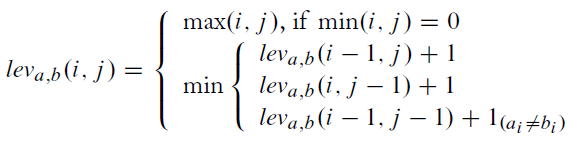
\includegraphics[width=13cm]{./figures/LevenshteinDistance.PNG}
	\caption[Levenshtein Distance]{Levenshtein Distance \cite{VassilisChristophides2015EntityRI-P25-28}}
	\label{fig:Levenshtein Distance}
	\end{center}
\end{figure}

\begin{figure}
	\begin{center}
	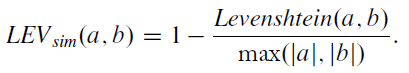
\includegraphics[width=13cm]{./figures/LevenshteinSimilarity.PNG}
	\caption[Levenshtein Similarity]{Levenshtein Similarity \cite{VassilisChristophides2015EntityRI-P25-28}}
	\label{fig:Levenshtein Similarity}
	\end{center}
\end{figure}

\textit{Jaro.}

\textit{Jaro-Winkler.}

\textit{Hamming.}

% -------------------------------------------------------------------------------------------------------
\textbf{Token-based String Similarity Measures.}

% \textit{N-Gram-similarity.}
% \begin{equation*}
%    \bar{\sigma}(s, t) = \frac{|ngram(s, n) \cap ngram(t, n)|}{\mbox{min}(|s|, |t|) - n + 1}
% \end{equation*}

\textit{Jaccard.}

\textit{Cosine.}

% -------------------------------------------------------------------------------------------------------
\textbf{Hybrid String Similarity Measures.}

\textit{Monge-Elkan.}

\textit{Soft TF-IDF.}

% -------------------------------------------------------------------------------------------------------
\textbf{Phonetic String Similarity Measures.}

% -------------------------------------------------------------------------------------------------------
\textbf{Embedding-based String Similarity Measures.}

\textit{BERT.}

\textit{fastText.}

% -------------------------------------------------------------------------------------------------------
\textbf{Datatype-specific String Similarity Measures.}

\textit{Sets of entities.}

\section{Data Fusion}

Data Fusion overcomes contradictory attribute values from different sources \cite{Bleiholder2009DataF}.